% https://www.geogebra.org/m/xr6nVvt4
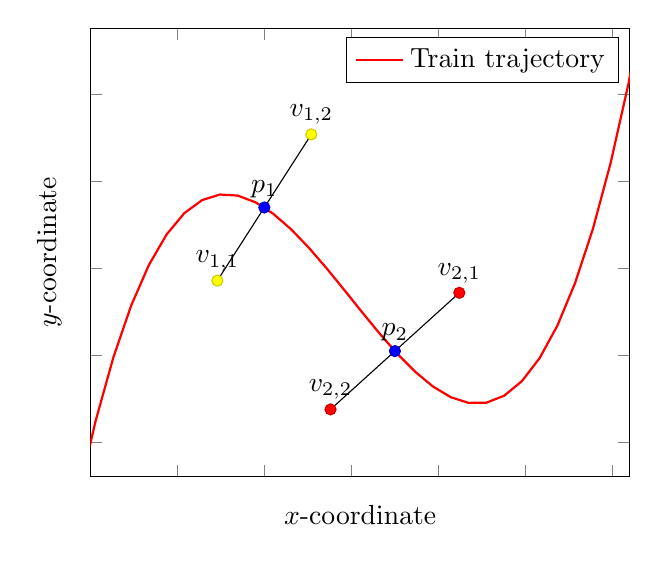
\begin{tikzpicture}
\begin{axis}[
    unit vector ratio=1 1 1,
    xmin=-2, xmax=4.2,
    %ymin=2, ymax=9,
    samples=50, 
    xlabel={$x$-coordinate}, ylabel={$y$-coordinate},
    xticklabels={,,},yticklabels={,,}]
\addplot[
    thick,
    red
] (x, 0.2*x*x*x-0.6 *x *x -0.65 *x + 2.7);
\addlegendentry{Train trajectory}

\addplot[
    scatter,
    mark=*, only marks,
    point meta=\thisrow{color},
    nodes near coords*={\annotvalue},
    visualization depends on={value \thisrow{label} \as \annotvalue},	
] table [] {
   x y color label
   0.00 2.70 1 $p_1$
   1.50 1.05 1 $p_2$
};

\addplot[
    scatter,
    mark=*,
    point meta=\thisrow{color},
    nodes near coords*={\annotvalue},
    visualization depends on={value \thisrow{label} \as \annotvalue},	
] table [] {
   x y color label
    -0.54 1.86 2 $v_{1,1}$
     0.54 3.54 2 $v_{1,2}$
};

\addplot[
    scatter,
    mark=*,
    point meta=\thisrow{color},
    nodes near coords*={\annotvalue},
    visualization depends on={value \thisrow{label} \as \annotvalue},
] table [] {
    x y color label
    2.24 1.72 4 $v_{2,1}$
    0.76 0.38 4 $v_{2,2}$

};

\end{axis}
\end{tikzpicture}